\chapter{Results}\label{results}
% Introduction: PAN20 uses these measures, so we do, too.
For the evaluation of our approaches we use several traditional as well as recently proposed measures.
\textcolor{olive}{(textbook citation needed for following definitions)} We use the convention that a pair is in the positive class iff both texts are written by the same author.
$tp$, $tn$, $fp$, $fn$ stand for the number of cases that where classified correctly as positive (true positives), correctly as negative (true negatives), falsely as positive (false positives) and falsely as negative (false negatives) respectively.\\
% Explain OOF cross-validation
% Precision
The \textbf{precision} $pre = \frac{tp}{tp+fp}$ of a classifier is the percentage of correct positive classifications $tp$ over all classifications $tp+fp$.
Thus, a precision approaching 1 indicates that an AV classifier's same-author predictions are near fully correct, meaning that there are nearly no false positives.\\
% Recall
The \textbf{recall} $rec = \frac{tp}{tp+fn}$ of a classifier is the percentage of correctly classified positive samples $tp$ over all positive samples $tp+fn$.
The lower the recall, the fewer same-author cases are recognized and predicted as such by an AV classifier.
In turn, a recall of 1 indicates that all same-author cases have been correctly identified.\\
% F1
Ideally, we want a system that classifies all same-author cases and only those as positive.
To measure this behavior, the \textbf{F1-score} $F_1 = 2\cdot\frac{prec\cdot{}rec}{prec+rec}$ can be used.
If both, precision and recall, approach 1 the F1-score of an AV classifier also approaches its maximum of 1.
Note that the F1 score weights precision and recall equally.
Especially for forensic Authorship Verification applications though, a high precision is more important than a high recall, as same-author decisions might be used as evidence and therefore must be reliable.
Also, in our setup, the F1 score ignores true negatives and therefore does not give an insight into how well the classifier detects different-author cases correctly.
For this, the different-author class would need to be assigned the positive label.\\
To mitigate some of the problems of the measures above and to better assess AV classifier performance, we use two more recently introduced measures.
% C@1, Point: non-answers (0.5) are possible
To measure include same-author and different-author classifications in the evaluation, one could use the accuracy $acc = \frac{tp+tn}{n}$, where $n = tp+tn+fp+fn$ is the total number of cases.
However, as \cite{bevendorff2019unmaskingShortTexts} points out, the results are often uncertain.
Also, in real-world applications wrong answers might be worse than non-answers.
Therefore, to give classification systems the option to withhold answers for difficult-to-decide cases, we use the \textbf{c@1-score} introduced by \cite{penas2011c_at_1} and adopted by PAN.
It is defined as $c@1 = \frac{n_{ac}}{n}+\frac{n_{ac}}{n}\cdot{}\frac{n_u}{n} = \frac{1}{n}\cdot{}\left(n_{ac}+\frac{n_{ac}}{n}\cdot{}n_u\right)$ where $n$ is again the total number of cases, $n_{ac} = tp+tn$ is the number of accurately classified cases and $n_u$ is the number of undecided cases.
This way, undecided cases count towards the c@1-score as if they were answered with the accuracy of the decided cases.
When an AV classifier gives an answer to all cases, the C@1-score is equivalent to the accuracy of the classifier.
A system that leaves all cases unanswered, receives a score of 0.\\
% F0.5u
Lastly, we use the \textbf{F0.5u-score} introduced by \cite{bevendorff2019unmaskingShortTexts}.
It is defined as $F_{0.5u} = \frac{(1+0.5^2)\cdot{}n_{tp}}{(1+0.5^2)\cdot{}n_{tp}+0.5^2\cdot{}(n_{fn}+n_u)+n_{fp}}$.
As mentioned above, a high precision result is more reliable than a high recall one.
To take this into consideration, the F0.5u-score weights precision two times as much as recall.
In addition, it also allows the classifiers to give non-answers.
However, as unanswered cases are often not useful in real-world applications, it interprets them as wrong answers.
Thus, the F0.5u-score highly emphasizes on the precision of an AV classifier.\\

% PAN20 measures:     AUC, C@1, F0.5u, F1, overall
% Unmasking measures: Precision, Recall, C@1, F0.5u


The results of our experiments can be seen in figures~\ref{tab:p_unmasking_gb}, \ref{tab:p_teahan_ff} and \ref{tab:p_teahan_gb}.
The tables show the absolute values for the transcription systems employed and their statistical significance compared to verbatim text in the first row.
The thresholds we use for statistical significance are:
\begin{itemize}
    \item $*$: statistically significant ($p < 0.05$)
    \item $*\! *$: very statistically significant ($p < 0.01$)
    \item $*\! *\! *$: highly statistically significant ($p < 0.001$)
\end{itemize}
Additionally, $+$ marks an increase and $-$ marks a decrease compared to the top row.
For example, $0.5936^{*\! *}_{-}$ indicates a very statistically significant decrease of the current transcription's performance compared to verbatim text.


% Unmasking
% - still variance is high, needs about 9%? to be significant
First, we will discuss the results of the Unmasking approach using the Gutenberg dataset.
Before analyzing the final results, let us take a look at the sets of the degradation curves generated through Unmasking.
The curve sets generated for each transcription can be split into five types depending on how fast the accuracy drops. % correlating to the number of types present in the transcription.
For $Verbatim$, $IPA$, $ASJP$, $Dolgo$, $RefSoundex$, $Metaphone$, $Soundex$, $P$, and $PL$, the curve degrades over the entirety of the iterations, giving the maximal resolution for further use as features.
Figure~\ref{fig:verbatim_curves} shows this ``best-case'' resolution for $Verbatim$.
Next, the curves for $IPA$ $4$-$grams$, $ASJP$ $4$-$grams$, $P$ $4$-$grams$, and $Dolgo$ $4$-$grams$ degrade quicker as can be seen in figure \ref{fig:ipa_4grams_curves} for $IPA$ $4$-$grams$.
This may be caused by a reduction of author-distinguishing features through $4$-$gram$-generation.
We suspect that -- analogous to stop words as discussed in chapter~\ref{related_work} -- certain of the possible $4$-$grams$ appear often and are suited well for distinguishing between authors while the following ones are not, resulting in a faster curve degradation.
Further investigation is needed to confirm or deny this hypothesis.
For $CV$ $4$-$grams$ (fig.~\ref{fig:cv_4grams_curves}) the accuracy drops to zero within very few Unmasking iterations, for the simple reason that it only contains 16 different types that are used as features.
The standard $CV$ transcription exhibits more chaotic curves, as shown in figure~\ref{fig:cv_curves}.
Apparently, a binary alphabet does not give the linear SVMs enough information to make robust guesses during curve generation.
Lastly, for $PLS$ (fig. \ref{fig:pls_curves}) the additional stop word removal leads to a much slower accuracy degradation.
As discussed earlier, stopwords are good features for distinguishing between authors.
Removing these common words results in the remaining features being more topic-related.
Thus, the given texts can be distinguished more easily even after removing certain of the remaining features.
As our goal, however, is not to retain a high accuracy of the curves, but to increase the differences between same-author and different-author curves, omitting stop words does not seem promising.\\
The results of the cross-validation for Unmasking using the Gutenberg dataset can be seen in figure~\ref{tab:p_unmasking_gb}.
As mentioned in chapter~\ref{sec:unmasking-approach}, Unmasking does not produce $non$-$answers$ and thus F0.5u is reduced to F0.5 and c@1 is equal to the classifier's accuracy.
The results of the individual folds have a high variance, characteristic of the probabilistic nature of Unmasking.
This is reflected in the results as the smallest change accepted as statistically significant ($p<0.05$) is the decrease of $c@1$ for $P$ $4$-$grams$ of 4.88\% from 0.6875 to 0.6387.
Generally, all statistically significant changes result in a reduction of performance with $CV$, $CV$ $4$-$grams$, and $IPA$ $4$-$grams$ reducing the performance the most overall.
As already discussed above, the Unmasking curves for $CV$ and $CV$ $4$-$grams$ exhibit characteristics suggesting a decrease in performance as the linear SVMs employed in the meta-classification do not have enough information to produce meaningful predictions.
For $IPA$ $4$-$grams$ the increase in vocabulary size to 350\% its original size probably results in too many features, also decreasing classifier performance.
To acquire a sense for range of performance reduction, figure~\ref{fig:results_f1_gb_unmasking} shows the F1-score achieved by each of the transcription systems.
A slight trend can be observed regarding the granularity of the transcription systems and their F1-score.
The broader the system, the worse it performs.
In general, $4$-$grams$ seem to perform worse then the transcriptions they were generated from.
Still, these observations have to be taken cautiously as most of the changes are not statistically significant.
Note that, although not statistically significant, $PL$ increases the all scores the most, suggesting that punctuation removal and lemmatization are a more promising pre-processing step.\\


\begin{figure}
  \centering
  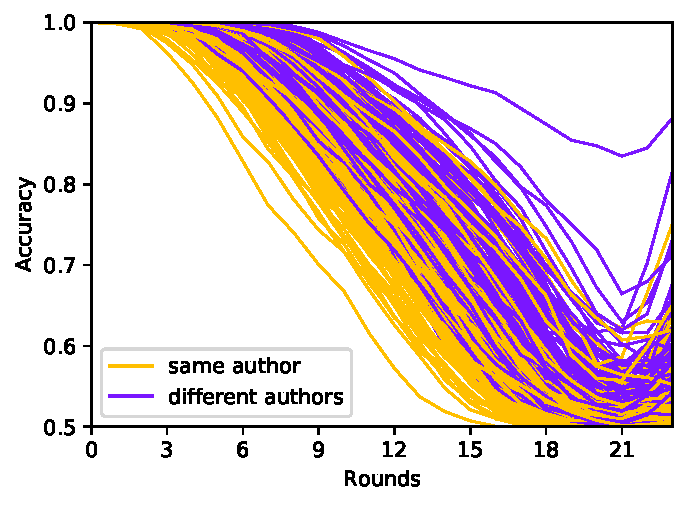
\includegraphics[width=0.7\textwidth]{figures/verbatim_curves}
  \caption{Unmasking curves for $Verbatim$ using the Gutenberg dataset}
  \label{fig:verbatim_curves}
\end{figure}
\begin{figure}
  \centering
  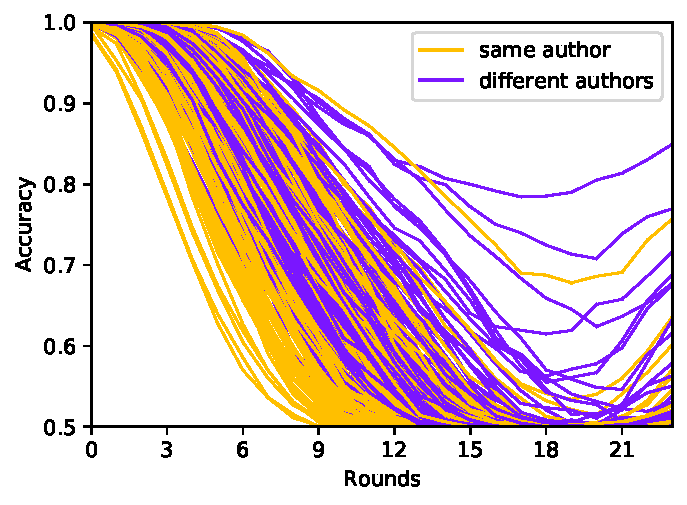
\includegraphics[width=0.7\textwidth]{figures/ipa_4grams_curves}
  \caption{Unmasking curves for $IPA$ $4$-$grams$ using the Gutenberg dataset}
  \label{fig:ipa_4grams_curves}
\end{figure}
\begin{figure}
  \centering
  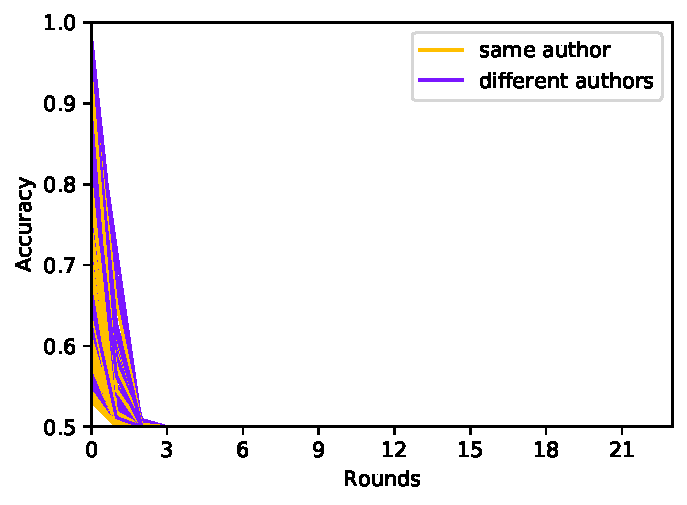
\includegraphics[width=0.7\textwidth]{figures/cv_4grams_curves}
  \caption{Unmasking curves for $CV$ $4$-$grams$ using the Gutenberg dataset}
  \label{fig:cv_4grams_curves}
\end{figure}
\begin{figure}
  \centering
  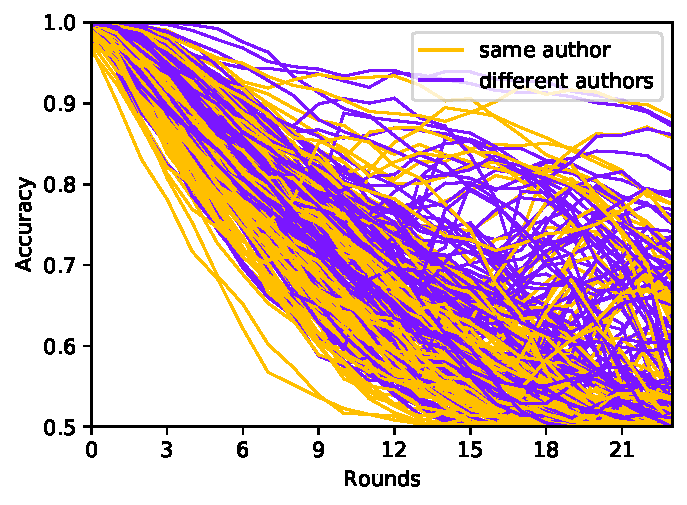
\includegraphics[width=0.7\textwidth]{figures/cv_curves}
  \caption{Unmasking curves for $CV$ using the Gutenberg dataset}
  \label{fig:cv_curves}
\end{figure}
\begin{figure}
  \centering
  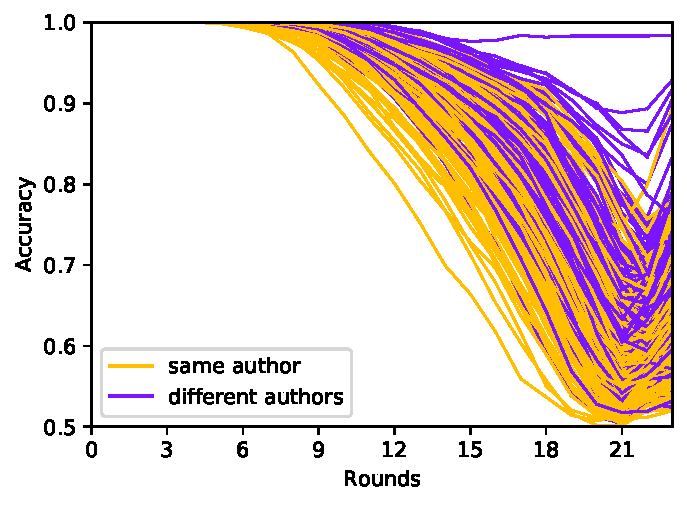
\includegraphics[width=0.7\textwidth]{figures/pls_curves}
  \caption{Unmasking curves for $PLS$ using the Gutenberg dataset}
  \label{fig:pls_curves}
\end{figure}
\begin{figure}
  \centering
  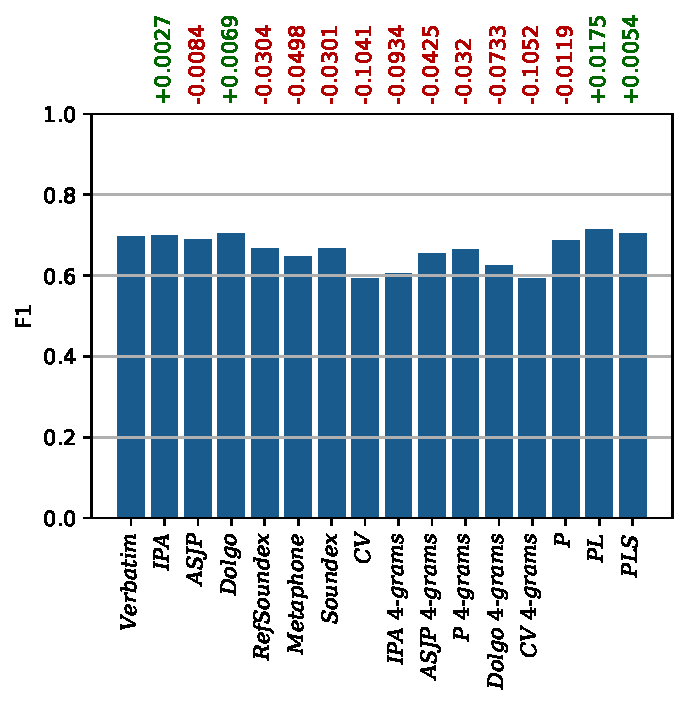
\includegraphics[width=0.7\textwidth]{figures/results_f1_gb_unmasking}
  \caption{F1-score and differences for Unmasking using the Gutenberg dataset, significant changes: $Metaphone^{*}$, $CV^{*\! *}$, $IPA$ $4$-$grams^{*\! *}$, and $CV$ $4$-$grams^{*\! *}$.}
  \label{fig:results_f1_gb_unmasking}
\end{figure}
\begin{figure}
  \centering
  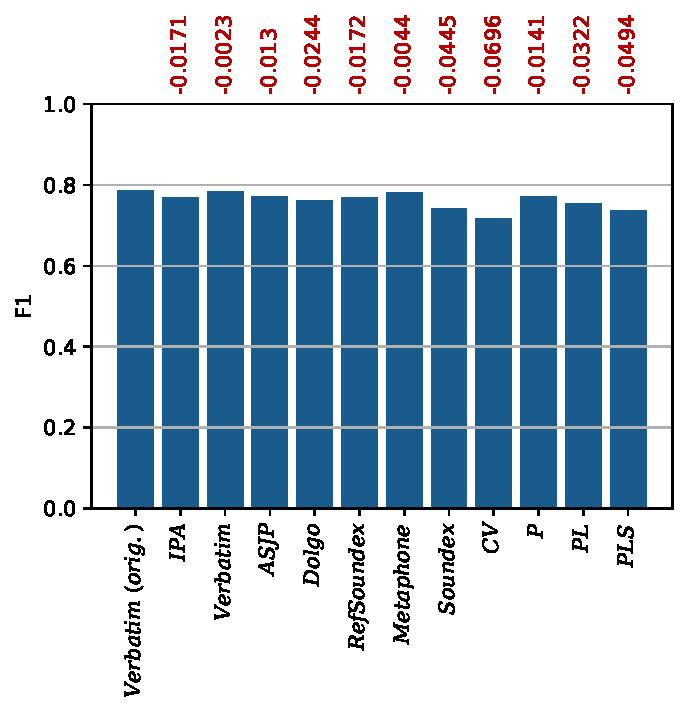
\includegraphics[width=0.7\textwidth]{figures/results_f1_ff_teahan}
  \caption{F1-score and differences for the compression approach using the Fan-fiction dataset, all changes are highly statistically significant.}
  \label{fig:results_f1_ff_teahan}
\end{figure}


% Then: Teahan Compression, Fan-fiction
The results of the compression approach using the Fan-fiction dataset provide a different picture.
As the cleaning step of the Fan-fiction dataset is phonetically-informed, we use the original data for comparison.
As can be seen in table~\ref{tab:p_teahan_ff}, almost all of the changes are statistically significant.
This is a result of the compression approach being deterministic and all variations being introduced by different configurations of cross-validation folds.
The practical significances of the results, however, are low.
Again, almost all experiments result in a decreased perfomance of the respective score.
Surprisingly, $Metaphone$ breaks this rule, yielding slight increases over $Verbatim$ text.
Its classification precision improves upon the baseline by 0.85\% leading to an improvement in F0.5u of 1.26\%.
$CV$ results in a minor improvement of 0.8\% in recall, but a major loss of 12.64\% in precision.
Figure~\ref{fig:results_f1_ff_teahan} shows the F1-score for this experiment.
The trend of broader transcriptions leading to worse performance can be observed here as well, with the highest drop of 6.96\% in F1 coming from $CV$.\\
As mentioned in chapter~\ref{sec:compression-approach}, we use the default uncertainty interval of [0.45,~0.55].
Increasing this interval improves precision and recall, because $non$-$answers$ are omitted in their calculation and thus only those answers are counted that the classifier is more certain of.
On the other hand, $F0.5u$ deteriorates as it counts $non$-$answers$ as wrong classifications.
Decreasing the uncertainty interval, on the other hand, leads to a general decrease in performance as uncertain answers are binarized and counted with the same weight as certain answers.\\

% Teahan Compression, Gutenberg
Lastly, table~\ref{tab:p_unmasking_gb} shows the results for the compression approach using the Gutenberg dataset.
During the cross-validation for this experiment, regardless of the number of splits, the classifier returned only negative classifications for some folds of the following transcriptions: $Dolgo$, $RefSoundex$, $Soundex$, $CV$, $ASJP$ $4$-$grams$, $P$ $4$-$grams$, $Dolgo$ $4$-$grams$, and $CV$ $4$-$grams$.
We suspect this happens because the broader transcriptions reduce the information in and already small dataset even further.
Subsequently, this circumstance weakens the validity of the results of this experiment overall.
Still, except a surprising improvement from $Metaphone$ by 7.31\% in precision, all other all significant results are decreasing the performance of $Verbatim$ text.
As the c@1-score of $Metaphone$ is reduced by 23.62\%, the most probable explanation for its raise in precision is that it produced many predictions within the uncertainty interval, which are omitted in the determination of the precision score.\\

Taking into account the results from all three experiments, we conclude that phonetically transcribing texts before using them in Authorship Verification does \textit{not} increase the performance of Unmasking and the compression approach by any practically significant amount.
Regarding the question whether a transcription systems granularity is correlated to its output, in the range of perfomance reduction, a slight trend can be seen:
Methods that produce extreme amounts of tokens -- very many such as $IPA$ $4$-$grams$ as well as very few such as $CV$ $4$-$grams$ -- perform worse than their more moderate counterparts.\\
In the following, we will discuss a number of possible reasons for the overall negative trend that phonetic transcriptions bring to the results.\\
Converting graphemes to phonemes, in our case verbatim text to its $IPA$ transcription, is a difficult task.
Moreover, when transcribing automatically, the transcription algorithm does not have any information about the pronunciation of the speaker of a given text.
Thus, usually text is transcribed to either the General (North) American pronunciation or the Received Pronunciation\footnote{British English}.
We use g2pE by \cite{kyubyong2019g2pE} which employs the Carnegie Mellon University Pronouncing Dictionary to look up transcriptions for words.
The CMU dictionary uses North American English as its pronunciation standard.
Thus, by transcribing we assume that the author has a North American English phonetic preference.
Transcribing, for example, both an Irish author's and a Nigerian author's texts to American English, one can imagine that a lot of phonetically relevant information, that could be used to distinguish them, is lost.
In the same vein, authors might \textit{actively} make efforts to impart certain phonetic qualities into their texts that are based on topic rather than the author's unconscious phonetic preference.
This becomes especially clear when an author uses direct speech, which often occurs in the datasets we use as they are both based on sets of fictional stories.
The ``voice in the author's head'' when writing a direct speech passage presumably varies greatly depending on the traits of the character depicted in the story.
Thus, extracting these features might aid in topic or genre identification more so than in Authorship Verification.
To mitigate this, direct speech could be removed from text entirely.\\
Another limitation of phonetic transcriptions for Authorship Analysis is due to the low-level nature they work at.
An author's freedom of self-expression is limited on the sub-segmental level, i.e., concerning individual sounds.
Usually, the meaning of a word changes together with its pronunciation.
The only words for which this is not the case are synonyms such as the words ``begin'' and ``star''.
Thus, authors that want to express similar ideas arguably will sound similar on the sub-segmental level not because of their phonetic preference but due to the proximity of the topics.
More importantly, if authors want to express different ideas the resulting transcriptions will also be different, without the Authorship Verification classifier knowing if this difference stems from two unique authors with varied phonetic preferences or from one author discussing different topics.
Supra-segmental features such as stress or prose can be utilized more freely and might give a more informative base for Authorship Analysis.\\
Lastly, standard Unmasking without using $n$-grams works on the lexical level, i.e., it uses entire words as atomic units and ignores the information encoded by the symbols inside a word.
With the step of transcription, however, we are precisely attempting to enhance this inner-word information.
Thus, for Unmasking the transcription of data serves only as a phonetically-informed binning method for types.
In an effort mitigate this, we used the $n$-gram based transcription method, which still led to negative results.\\


% Problem 3 / Following thoughts: Phonetic transcriptions / features are probably bad Authorship predictors but better predictors for other features such as genre, topic, age of setting.
\begin{table}
\caption{Results for Unmasking using the Gutenberg dataset with Bonferroni-corrected significance markers.}
\label{tab:p_unmasking_gb}
\centering\small
\begin{tabular}{@{}l@{\hspace{1\tabcolsep}}lllll@{}} % Use @{\hspace{2\tabcolsep}} to double the spacing
\toprule
\bf System & \bf Precision & \bf Recall & \bf F1 & \bf F0.5u (F0.5) & \bf c@1 (Accuracy) \\
\midrule
$Verbatim$ & $0.7545$ & $0.6539$ & $0.6977$ & $0.6784$ & $0.6875$ \\
\midrule
$IPA$ & $0.7537$ & $0.6701$ & $0.7004$ & $0.6641$ & $0.6833$ \\
$ASJP$ & $0.7284$ & $0.667$ & $0.6893$ & $0.6455$ & $0.676$ \\
$Dolgo$ & $0.7551$ & $0.6733$ & $0.7046$ & $0.6617$ & $0.6792$ \\
$RefSoundex$ & $0.7297$ & $0.6275$ & $0.6673$ & $0.6233^{*\! *}_{-}$ & $0.6542$ \\
$Metaphone$ & $0.7193$ & $0.6028$ & $0.648^{*}_{-}$ & $0.6143^{*\! *}_{-}$ & $0.6423^{*\! *}_{-}$ \\
$Soundex$ & $0.7333$ & $0.6363$ & $0.6677$ & $0.6234^{*\! *}_{-}$ & $0.6512$ \\
$CV$ & $0.6316^{*\! *}_{-}$ & $0.5757$ & $0.5936^{*\! *}_{-}$ & $0.5171^{*\! *\! *}_{-}$ & $0.5381^{*\! *\! *}_{-}$ \\
$IPA$ $4$-$grams$ & $0.6536^{*\! *}_{-}$ & $0.5814$ & $0.6043^{*\! *}_{-}$ & $0.5505^{*\! *\! *}_{-}$ & $0.5976^{*\! *\! *}_{-}$ \\
$ASJP$ $4$-$grams$ & $0.721$ & $0.6148$ & $0.6553$ & $0.6086$ & $0.6257$ \\
$P$ $4$-$grams$ & $0.718$ & $0.6339$ & $0.6658$ & $0.6207^{*}_{-}$ & $0.6387^{*}_{-}$ \\
$Dolgo$ $4$-$grams$ & $0.6894$ & $0.5964$ & $0.6245$ & $0.5558^{*\! *\! *}_{-}$ & $0.6012^{*\! *}_{-}$ \\
$CV$ $4$-$grams$ & $0.6161^{*\! *}_{-}$ & $0.5853$ & $0.5926^{*\! *}_{-}$ & $0.4868^{*\! *\! *}_{-}$ & $0.5151^{*\! *\! *}_{-}$ \\
$P$ & $0.7155$ & $0.6672$ & $0.6859$ & $0.6452$ & $0.6745$ \\
$PL$ & $\mathbf{0.7707}$ & $\mathbf{0.6801}$ & $\mathbf{0.7153}$ & $\mathbf{0.6876}$ & $\mathbf{0.7079}$ \\
$PLS$ & $0.7676$ & $0.6614$ & $0.7031$ & $0.6572$ & $0.6905$ \\
\bottomrule
\end{tabular}
\end{table}

\begin{table}
\caption{Results for the compression approach using the Fan-fiction dataset compared to $Verbatim$ text (uncleaned) with Bonferroni-corrected significance markers.}
\label{tab:p_teahan_ff}
\centering\small
\begin{tabular}{@{}l@{\hspace{1\tabcolsep}}lllll@{}} % Use @{\hspace{2\tabcolsep}} to double the spacing
\toprule
\bf System & \bf Precision & \bf Recall & \bf F1 & \bf F0.5u & \bf c@1 \\
\midrule
$Verbatim$ $(orig.)$ & $0.7635$ & $0.8092$ & $\mathbf{0.7856}$ & $0.714$ & $0.7431$ \\
\midrule
$IPA$ & $0.7532^{*\! *\! *}_{-}$ & $0.7846^{*\! *\! *}_{-}$ & $0.7686^{*\! *\! *}_{-}$ & $0.7098^{*\! *\! *}_{-}$ & $0.7291^{*\! *\! *}_{-}$ \\
$Verbatim$ & $0.7604^{*\! *\! *}_{-}$ & $0.8078^{*\! *}_{-}$ & $0.7833^{*\! *\! *}_{-}$ & $0.7101^{*\! *\! *}_{-}$ & $0.739^{*\! *\! *}_{-}$ \\
$ASJP$ & $0.7602^{*\! *}_{-}$ & $0.7857^{*\! *\! *}_{-}$ & $0.7727^{*\! *\! *}_{-}$ & $0.7148$ & $0.7353^{*\! *\! *}_{-}$ \\
$Dolgo$ & $0.7474^{*\! *\! *}_{-}$ & $0.7757^{*\! *\! *}_{-}$ & $0.7612^{*\! *\! *}_{-}$ & $0.6992^{*\! *\! *}_{-}$ & $0.7174^{*\! *\! *}_{-}$ \\
$RefSoundex$ & $0.7564^{*\! *\! *}_{-}$ & $0.7811^{*\! *\! *}_{-}$ & $0.7685^{*\! *\! *}_{-}$ & $0.7049^{*\! *\! *}_{-}$ & $0.7259^{*\! *\! *}_{-}$ \\
$Metaphone$ & $\mathbf{0.772}^{*\! *\! *}_{+}$ & $0.7907^{*\! *\! *}_{-}$ & $0.7813^{*\! *\! *}_{-}$ & $\mathbf{0.7266}^{*\! *\! *}_{+}$ & $\mathbf{0.7477}^{*\! *\! *}_{+}$ \\
$Soundex$ & $0.7129^{*\! *\! *}_{-}$ & $0.7717^{*\! *\! *}_{-}$ & $0.7411^{*\! *\! *}_{-}$ & $0.6758^{*\! *\! *}_{-}$ & $0.6839^{*\! *\! *}_{-}$ \\
$CV$ & $0.6371^{*\! *\! *}_{-}$ & $\mathbf{0.8172}^{*\! *}_{+}$ & $0.716^{*\! *\! *}_{-}$ & $0.6253^{*\! *\! *}_{-}$ & $0.5842^{*\! *\! *}_{-}$ \\
$P$ & $0.7528^{*\! *\! *}_{-}$ & $0.7914^{*\! *\! *}_{-}$ & $0.7716^{*\! *\! *}_{-}$ & $0.7092^{*\! *\! *}_{-}$ & $0.7304^{*\! *\! *}_{-}$ \\
$PL$ & $0.7228^{*\! *\! *}_{-}$ & $0.7868^{*\! *\! *}_{-}$ & $0.7534^{*\! *\! *}_{-}$ & $0.6782^{*\! *\! *}_{-}$ & $0.6949^{*\! *\! *}_{-}$ \\
$PLS$ & $0.6994^{*\! *\! *}_{-}$ & $0.7773^{*\! *\! *}_{-}$ & $0.7363^{*\! *\! *}_{-}$ & $0.6604^{*\! *\! *}_{-}$ & $0.668^{*\! *\! *}_{-}$ \\
\bottomrule
\end{tabular}
\end{table}


\begin{table}
\caption{Results for the compression approach using the Gutenberg dataset compared to $Verbatim$ text with Bonferroni-corrected significance markers.}
\label{tab:p_teahan_gb}
\centering\small
\begin{tabular}{@{}l@{\hspace{1\tabcolsep}}lllll@{}} % Use @{\hspace{2\tabcolsep}} to double the spacing
\toprule
\bf System & \bf Precision & \bf Recall & \bf F1 & \bf F0.5u & \bf c@1 \\
\midrule
$Verbatim$ & $0.871$ & $\mathbf{0.7354}$ & $0.7909$ & $0.6163$ & $\mathbf{0.645}$ \\
\midrule
$IPA$ & $0.8545$ & $0.676^{*}_{-}$ & $0.7383^{*}_{-}$ & $0.5951$ & $0.5396^{*\! *\! *}_{-}$ \\
$ASJP$ & $0.8738$ & $0.7241$ & $0.7786$ & $0.607$ & $0.5325^{*\! *\! *}_{-}$ \\
$Metaphone$ & $\mathbf{0.9441}^{*\! *}_{+}$ & $0.7265$ & $\mathbf{0.8005}$ & $0.5824^{*\! *}_{-}$ & $0.4088^{*\! *\! *}_{-}$ \\
$IPA$ $4$-$grams$ & $0.9117$ & $0.74$ & $0.7895$ & $0.5611^{*\! *\! *}_{-}$ & $0.3793^{*\! *\! *}_{-}$ \\
$P$ & $0.8816$ & $0.7178$ & $0.7801$ & $0.5979$ & $0.5655^{*\! *\! *}_{-}$ \\
$PL$ & $0.8664$ & $0.7237$ & $0.7734$ & $0.592^{*\! *}_{-}$ & $0.5554^{*\! *\! *}_{-}$ \\
$PLS$ & $0.8006$ & $0.7056$ & $0.737^{*}_{-}$ & $\mathbf{0.6165}$ & $0.6197$ \\
\bottomrule
\end{tabular}
\end{table}